\documentclass[UTF8,14pt]{article}
\usepackage[UTF8]{ctex}
\usepackage[a4paper, margin=0.8in,top = 20mm,bottom = 20mm]{geometry}
\usepackage{fancyhdr}
\usepackage{wrapfig}
\usepackage{subfigure,graphicx} % Required to insert images
\usepackage{enumitem}
\usepackage[colorlinks,linkcolor=black]{hyperref}
\usepackage{multicol}
\usepackage{listings}

% \numberwithin{figure}{subsubsection}
% \numberwithin{table}{subsubsection}
\pagestyle{fancy}
\lhead{天津英赛迪科技有限公司}
\chead{基于树莓派的步进电机图形化程序控制}
\rhead{谢远峰}
\renewcommand\headrulewidth{0.2pt}
% \renewcommand\footrulewidth{0.2pt}
\newcommand\sectionone[1]{\centerline{\Large{\bfseries{#1}}}}
\newcommand\sectiontwo[1]{\centerline{\large{\bfseries{#1}}}}
\setlength{\headsep}{4mm}
\setlength{\footskip}{5mm}


\setenumerate[1]{itemsep=0pt,partopsep=0pt,parsep=\parskip,topsep=0pt}
\setitemize[1]{itemsep=0pt,partopsep=0pt,parsep=\parskip,topsep=0pt}
\setdescription{itemsep=0pt,partopsep=0pt,parsep=\parskip,topsep=0pt}

\lstset{
    basicstyle          =   \sffamily,          % 基本代码风格
    keywordstyle        =   \bfseries,          % 关键字风格
    commentstyle        =   \rmfamily\itshape,  % 注释的风格,斜体
    stringstyle         =   \ttfamily,  % 字符串风格
    flexiblecolumns,                % 别问为什么,加上这个
    numbers             =   left,   % 行号的位置在左边
    showspaces          =   false,  % 是否显示空格,显示了有点乱,所以不现实了
    numberstyle         =   \zihao{-5}\ttfamily,    % 行号的样式,小五号,tt等宽字体
    showstringspaces    =   false,
    captionpos          =   t,      % 这段代码的名字所呈现的位置,t指的是top上面
    frame               =   lrtb,   % 显示边框
}

\lstdefinestyle{C}{
    language        =   C, % 语言选Python
    basicstyle      =   \zihao{-5}\ttfamily,
    numberstyle     =   \zihao{-5}\ttfamily,
    keywordstyle    =   \color{blue},
    keywordstyle    =   [2] \color{teal},
    stringstyle     =   \color{magenta},
    commentstyle    =   \color{red}\ttfamily,
    breaklines      =   true,   % 自动换行,建议不要写太长的行
    columns         =   fixed,  % 如果不加这一句,字间距就不固定,很丑,必须加
    basewidth       =   0.5em,
}


\Huge
\title{基于树莓派的步进电机图形化程序控制}
\begin{document}

\begin{titlepage}
	\begin{center}
		\begin{figure}
			\centering
			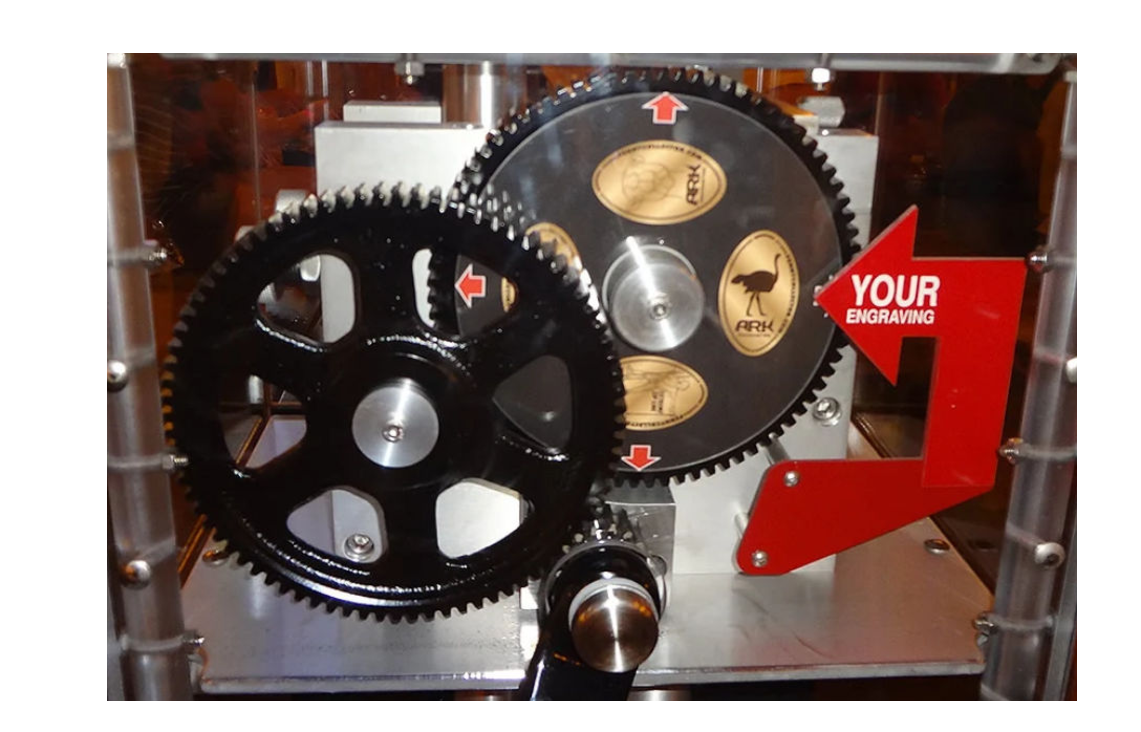
\includegraphics[width=8.2cm]{figures/压币机.pdf}
		\end{figure}
		\vspace{0.2cm}
		\begin{figure}
			\centering
			
\includegraphics[width=4.35cm]{figures/RPi-Logo-Reg-SCREEN.pdf}
		\end{figure}
		\vspace*{0.7cm}
		\line(1,0){300}\\
		[-0.2cm]
		\Huge{\bfseries 压币机程序设计}\\
		\vspace*{-0.7cm}
		\line(1,0){300}\\
		\LARGE {基于树莓派的步进电机图形化程序控制\\
			2021年7月22日}\\
		[0.6cm]
		\Large{
			\begin{tabular}{rl}
				单位:         & 天津英赛迪科技有限公司      \\
				姓名        : & 谢远峰                      \\
				时间       :  & 2021年7月22日——2021年8月6日
			\end{tabular}
		}
	\end{center}

\end{titlepage}
\clearpage
\sectionone{摘要}

压币机利用机械挤压的方式将硬币进行二次加工,形成一个细长硬币。
新硬币相对于传统硬币被压平或拉伸,并拥有新的设计压花。此类硬币常被用作
纪念品。在旅游园区中常见到压币机。



\vspace{0.5cm}
\sectionone{程序设计需求描述}

\begin{enumerate}
	\item 基于树莓派平台+可触摸屏幕(基于Python-tkinter库的图形化可执行界面程序)
	\item 进入程序主界面,显示印花、初始化、开始、使用说明选项
	\item 印花图案的选择(程序主页:显示四个图案,代表四种印花格式)
	\item 四个印花图案默认情况下为未选择模式,图案底部默认设置按钮颜色为红色(不选择)
	\item 点选印花图案后,按钮颜色由红色转换为绿色
	\item 用户进行纪念币打印之前,可点击使用说明进行程序使用流程的查看
	\item 选择印花图案后,点击初始化按钮,完成电机初始化
	\item 初始化完成后,出现初始化完成窗口,用户进行确认
	\item 用户确认初始化完毕后,用户点击开始按钮,程序驱动电机开始移动
	\item 打印完成后,出现打印完成,提醒用户拿取纪念币的窗口,等待用户确认
	\item 用户点击确认后,自动返回到程序主界面
\end{enumerate}

\vspace{0.5cm}
\sectionone{程序流程介绍}
\begin{wrapfigure}[20]{r}{0.4\textwidth}%靠文字内容的左侧
	\vspace{-0.4cm}
	\centering
	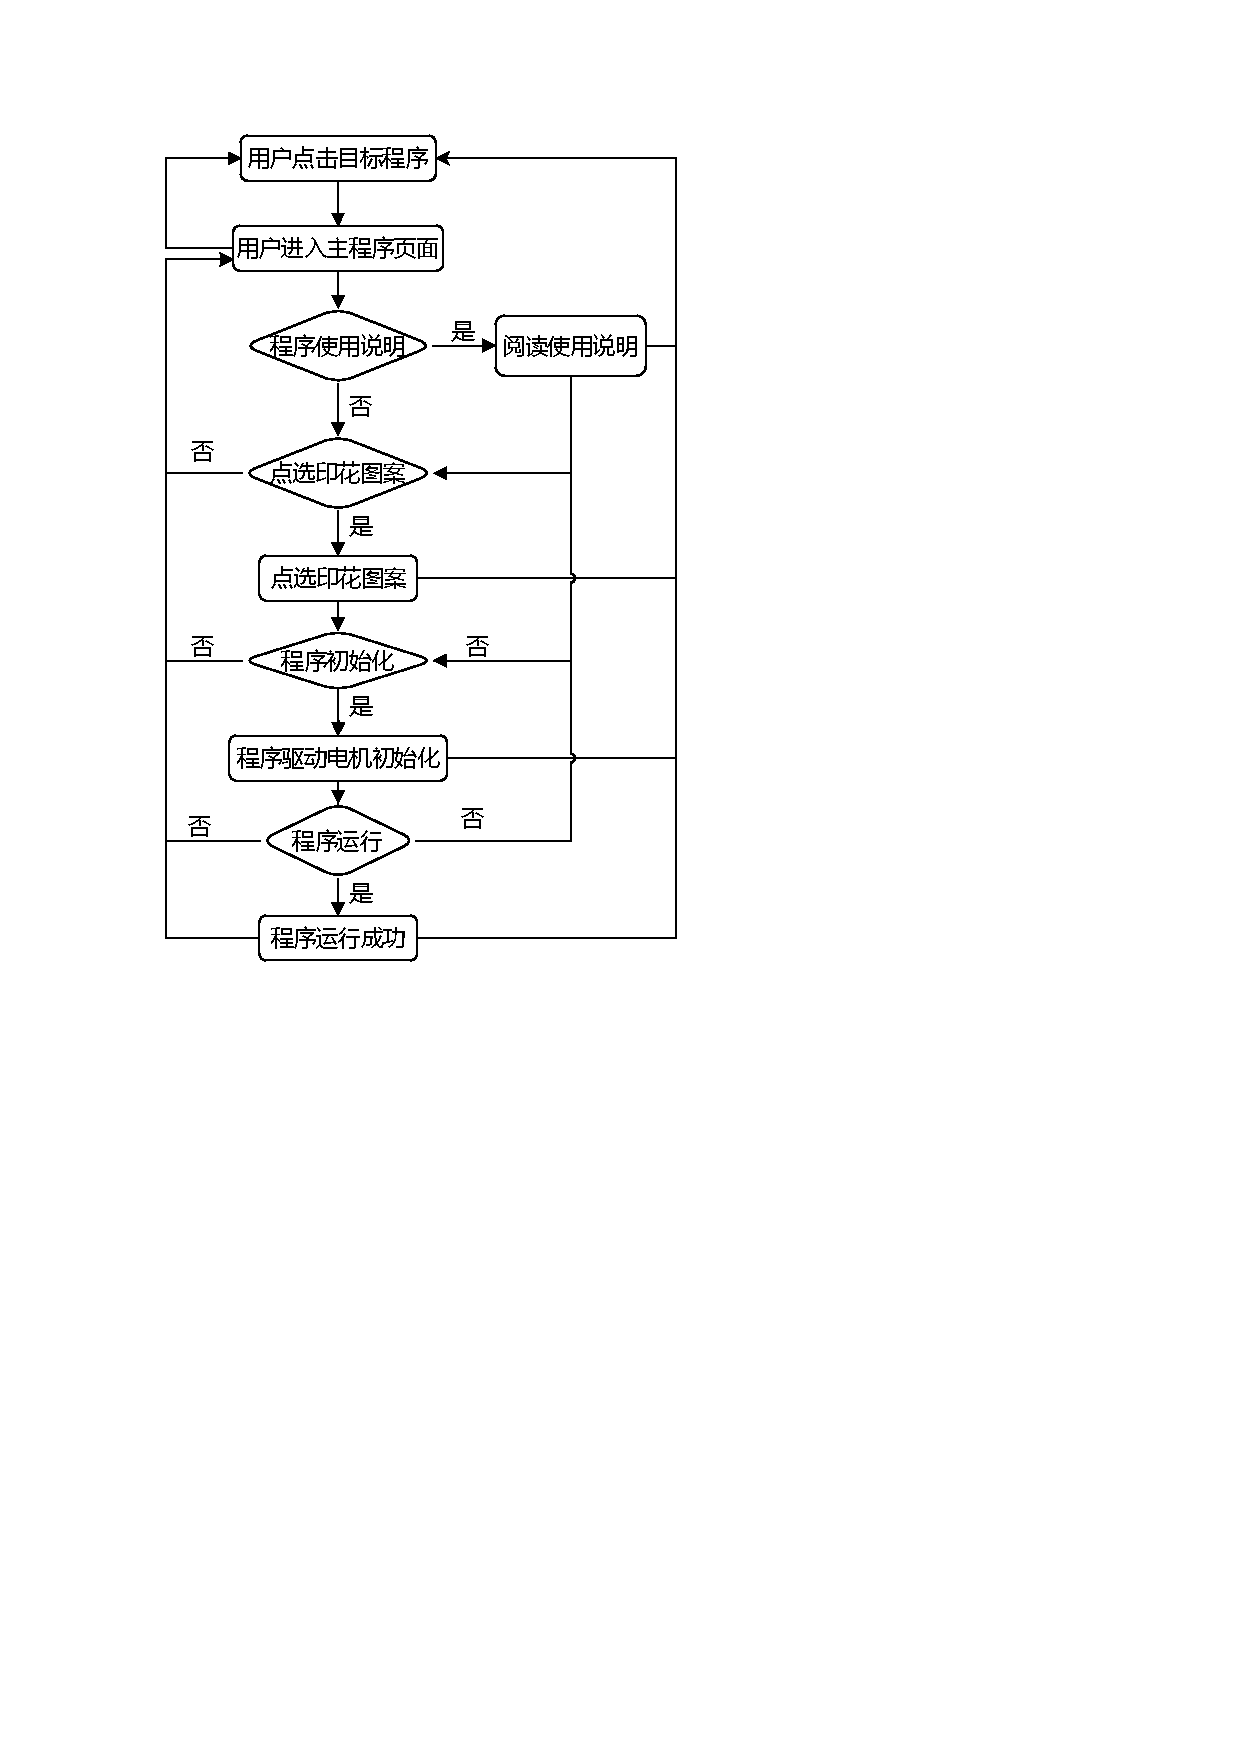
\includegraphics[width=6.56cm]{figures/流程图.pdf}
	\vspace{-10pt}
	\caption{程序运行流程图}
	\vspace{-15pt}
\end{wrapfigure}
程序常规流程图说明
\begin{enumerate}
	\item 用户点击目标可执行程序,进入程序主页面
	\item 用户点击使用说明,查看程序执行方式(选)
	\item 用户点击任一印花图案,印花图案下方按钮由红转绿
	\item 用户点击初始化按键,程序驱动电机进行初始化
	\item 程序返回初始化成功窗口,用户点击确认
	\item 用户点击开始按键,程序驱动电机进行硬币的印花压制
	\item 程序返回硬币制作成功的窗口,用户点击确认
	\item 用户拿取已制作好的纪念币
	\item 程序返回至默认初始化状态
\end{enumerate}

异常分支说明
\begin{enumerate}
	\item 用户进入程序主页面,关闭
	\item 用户未查看程序使用说明,直接进行程序初始化
	\item 用户选择印花图案后,未进行进一步操作
	\item 程序初始化失败
	\item 用户进行初始化后,未进行进一步操作
	\item 程序运行失败
	\item 程序初始化过程中关闭程序
	\item 程序运行过程中关闭程序
\end{enumerate}

\vspace{0.5cm}
\begin{figure}[!htbp]
	\centering
	\subfigure[初始化成功]{
		\begin{minipage}[t]{0.22\linewidth}
			\centering
			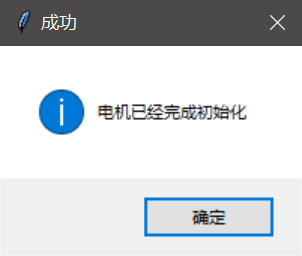
\includegraphics[width=1in]{figures/提示程序.png}
			%\caption{fig1}
		\end{minipage}%
	}
	\subfigure[初始化异常]{
		\begin{minipage}[t]{0.22\linewidth}
			\centering
			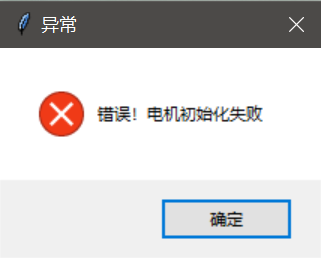
\includegraphics[width=1in]{figures/初始化异常.png}
			%\caption{fig2}
		\end{minipage}%
	}
	\subfigure[程序打印成功]{
		\begin{minipage}[t]{0.22\linewidth}
			\centering
			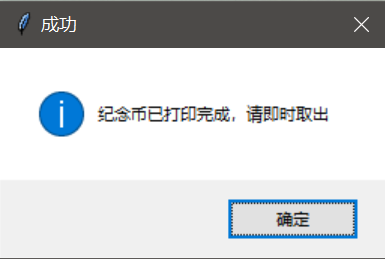
\includegraphics[width=1in]{figures/打印完成.png}
			%\caption{fig2}
		\end{minipage}
	}%
	\subfigure[程序打印异常]{
		\begin{minipage}[t]{0.22\linewidth}
			\centering
			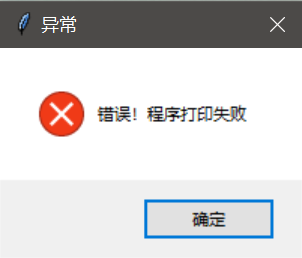
\includegraphics[width=1in]{figures/程序运行失败.png}
			%\caption{fig2}
		\end{minipage}
	}%
	\centering
	\caption{程序提示样例}
\end{figure}

\clearpage
\sectionone{附录}
\sectiontwo{A:针脚说明图}
\begin{figure}[!h]
	\centering
	\vspace{-10pt}
	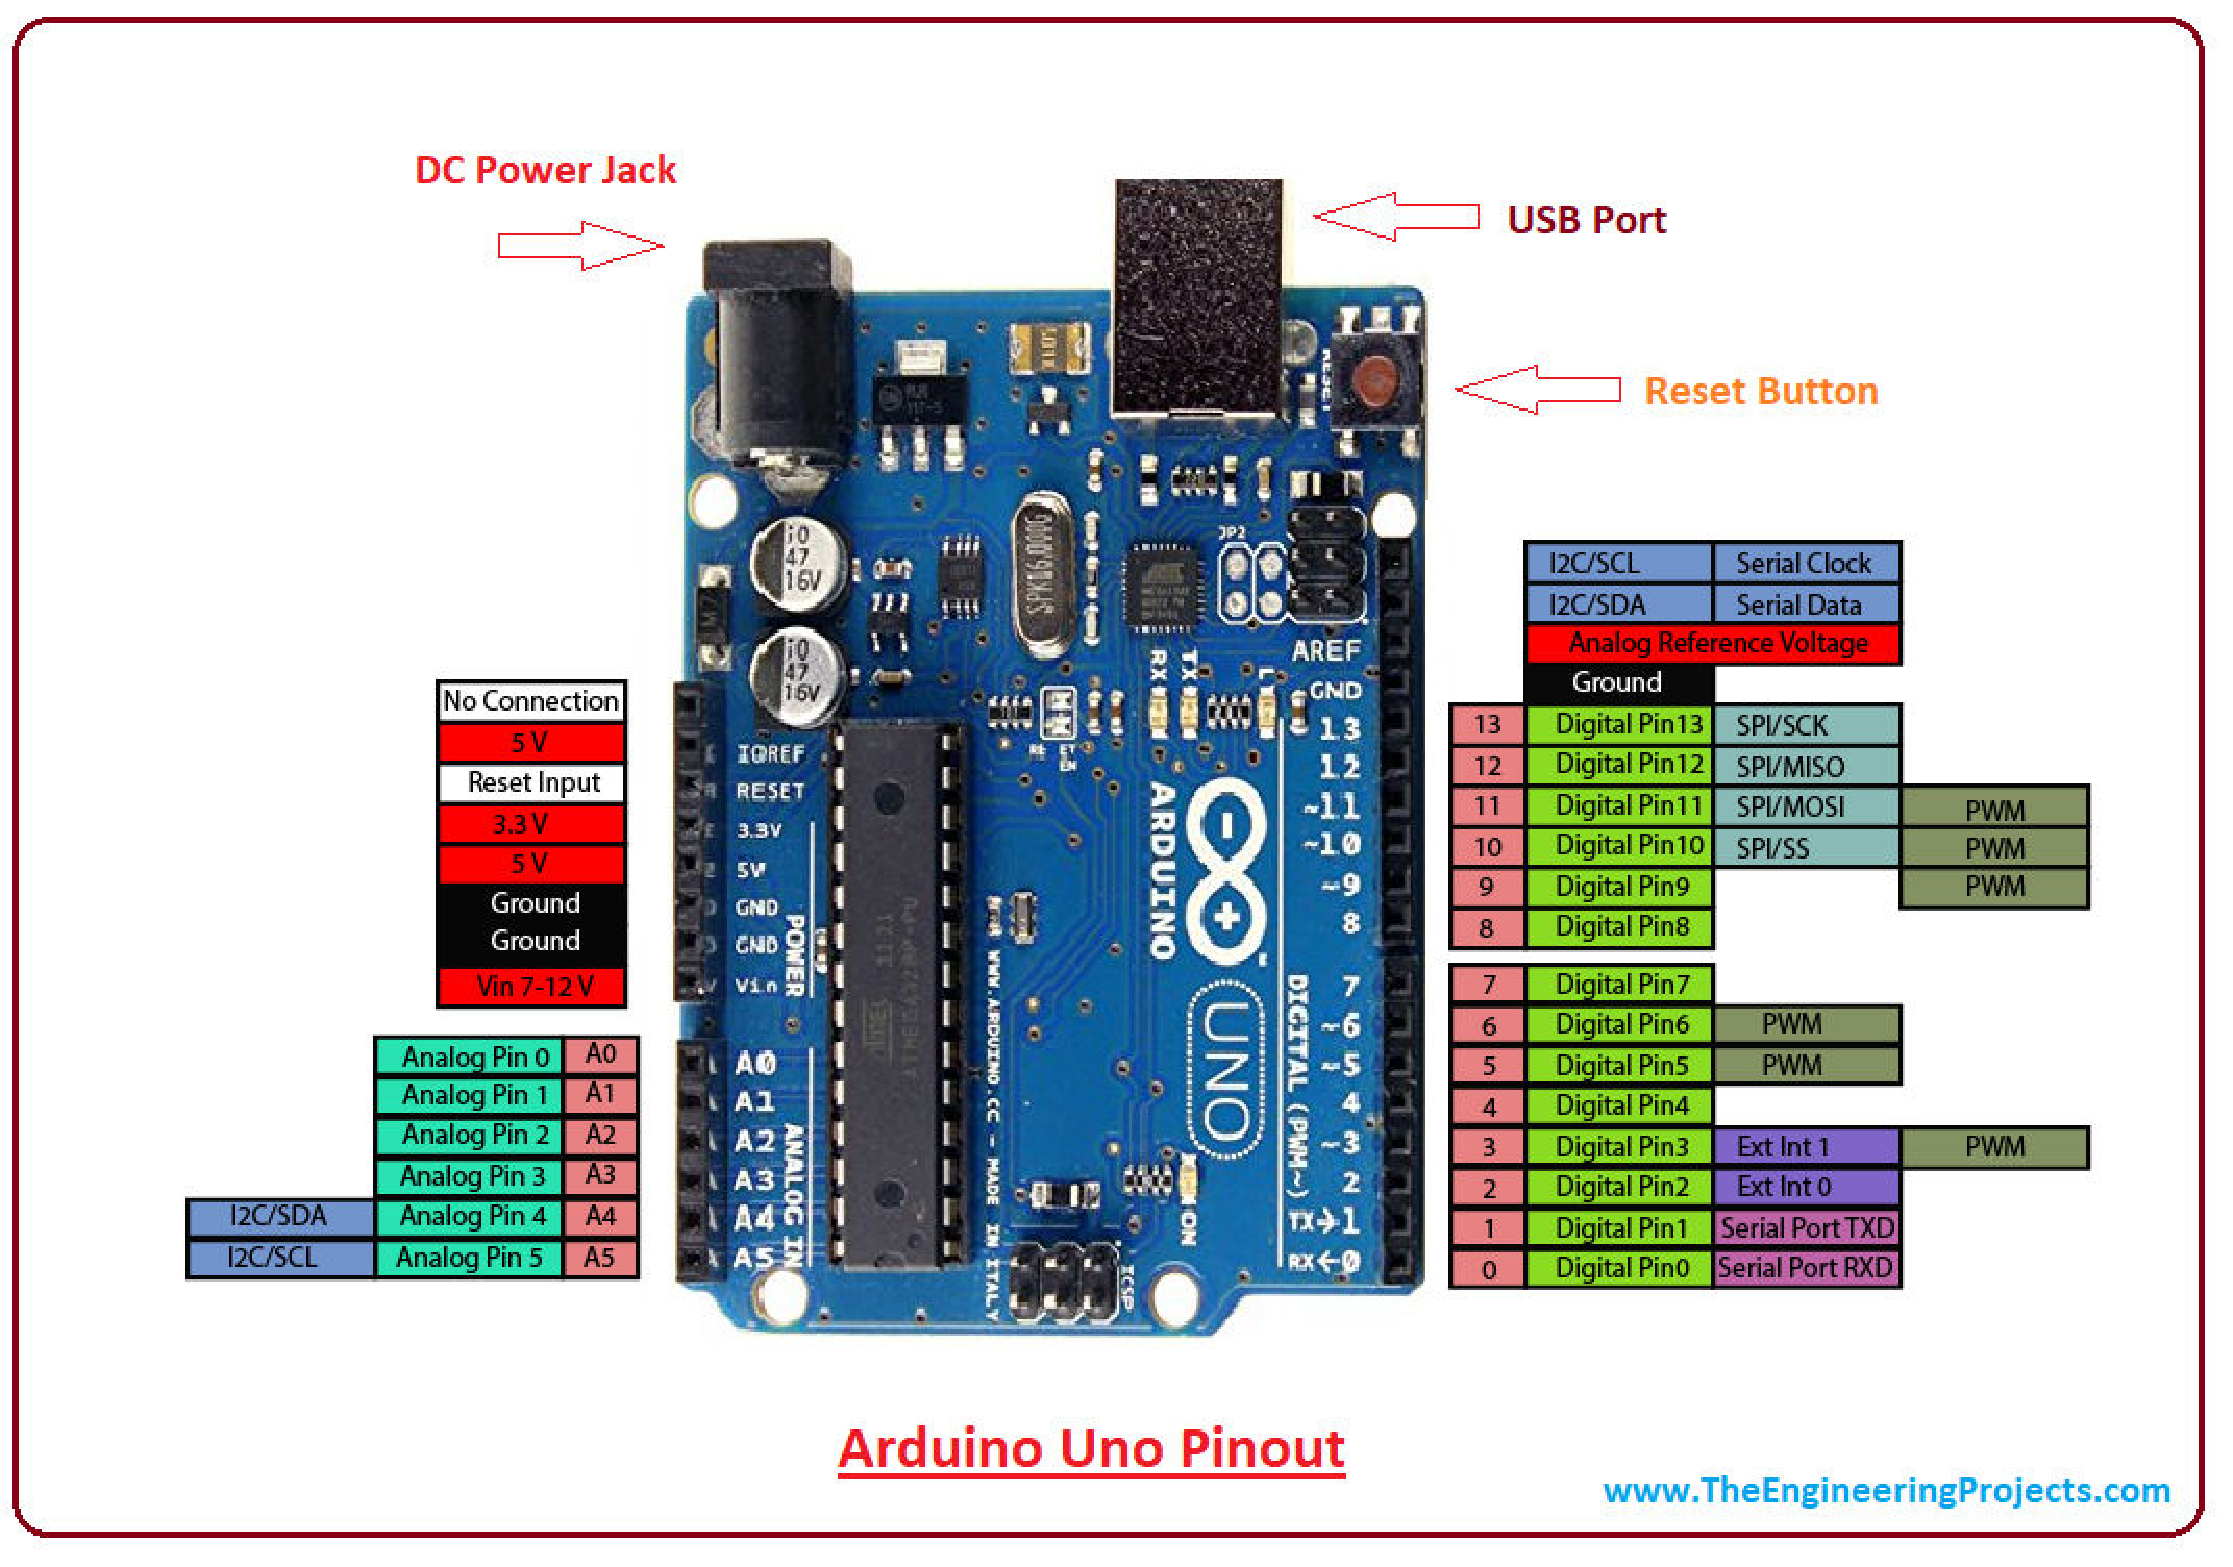
\includegraphics[width=15cm]{figures/arduino-uno.pdf}
	\vspace{-15pt}
	\caption{Arduino针脚}
	% \vspace{-15pt}
\end{figure}

\begin{figure}[!h]
	\centering
	% \vspace{-10pt}
	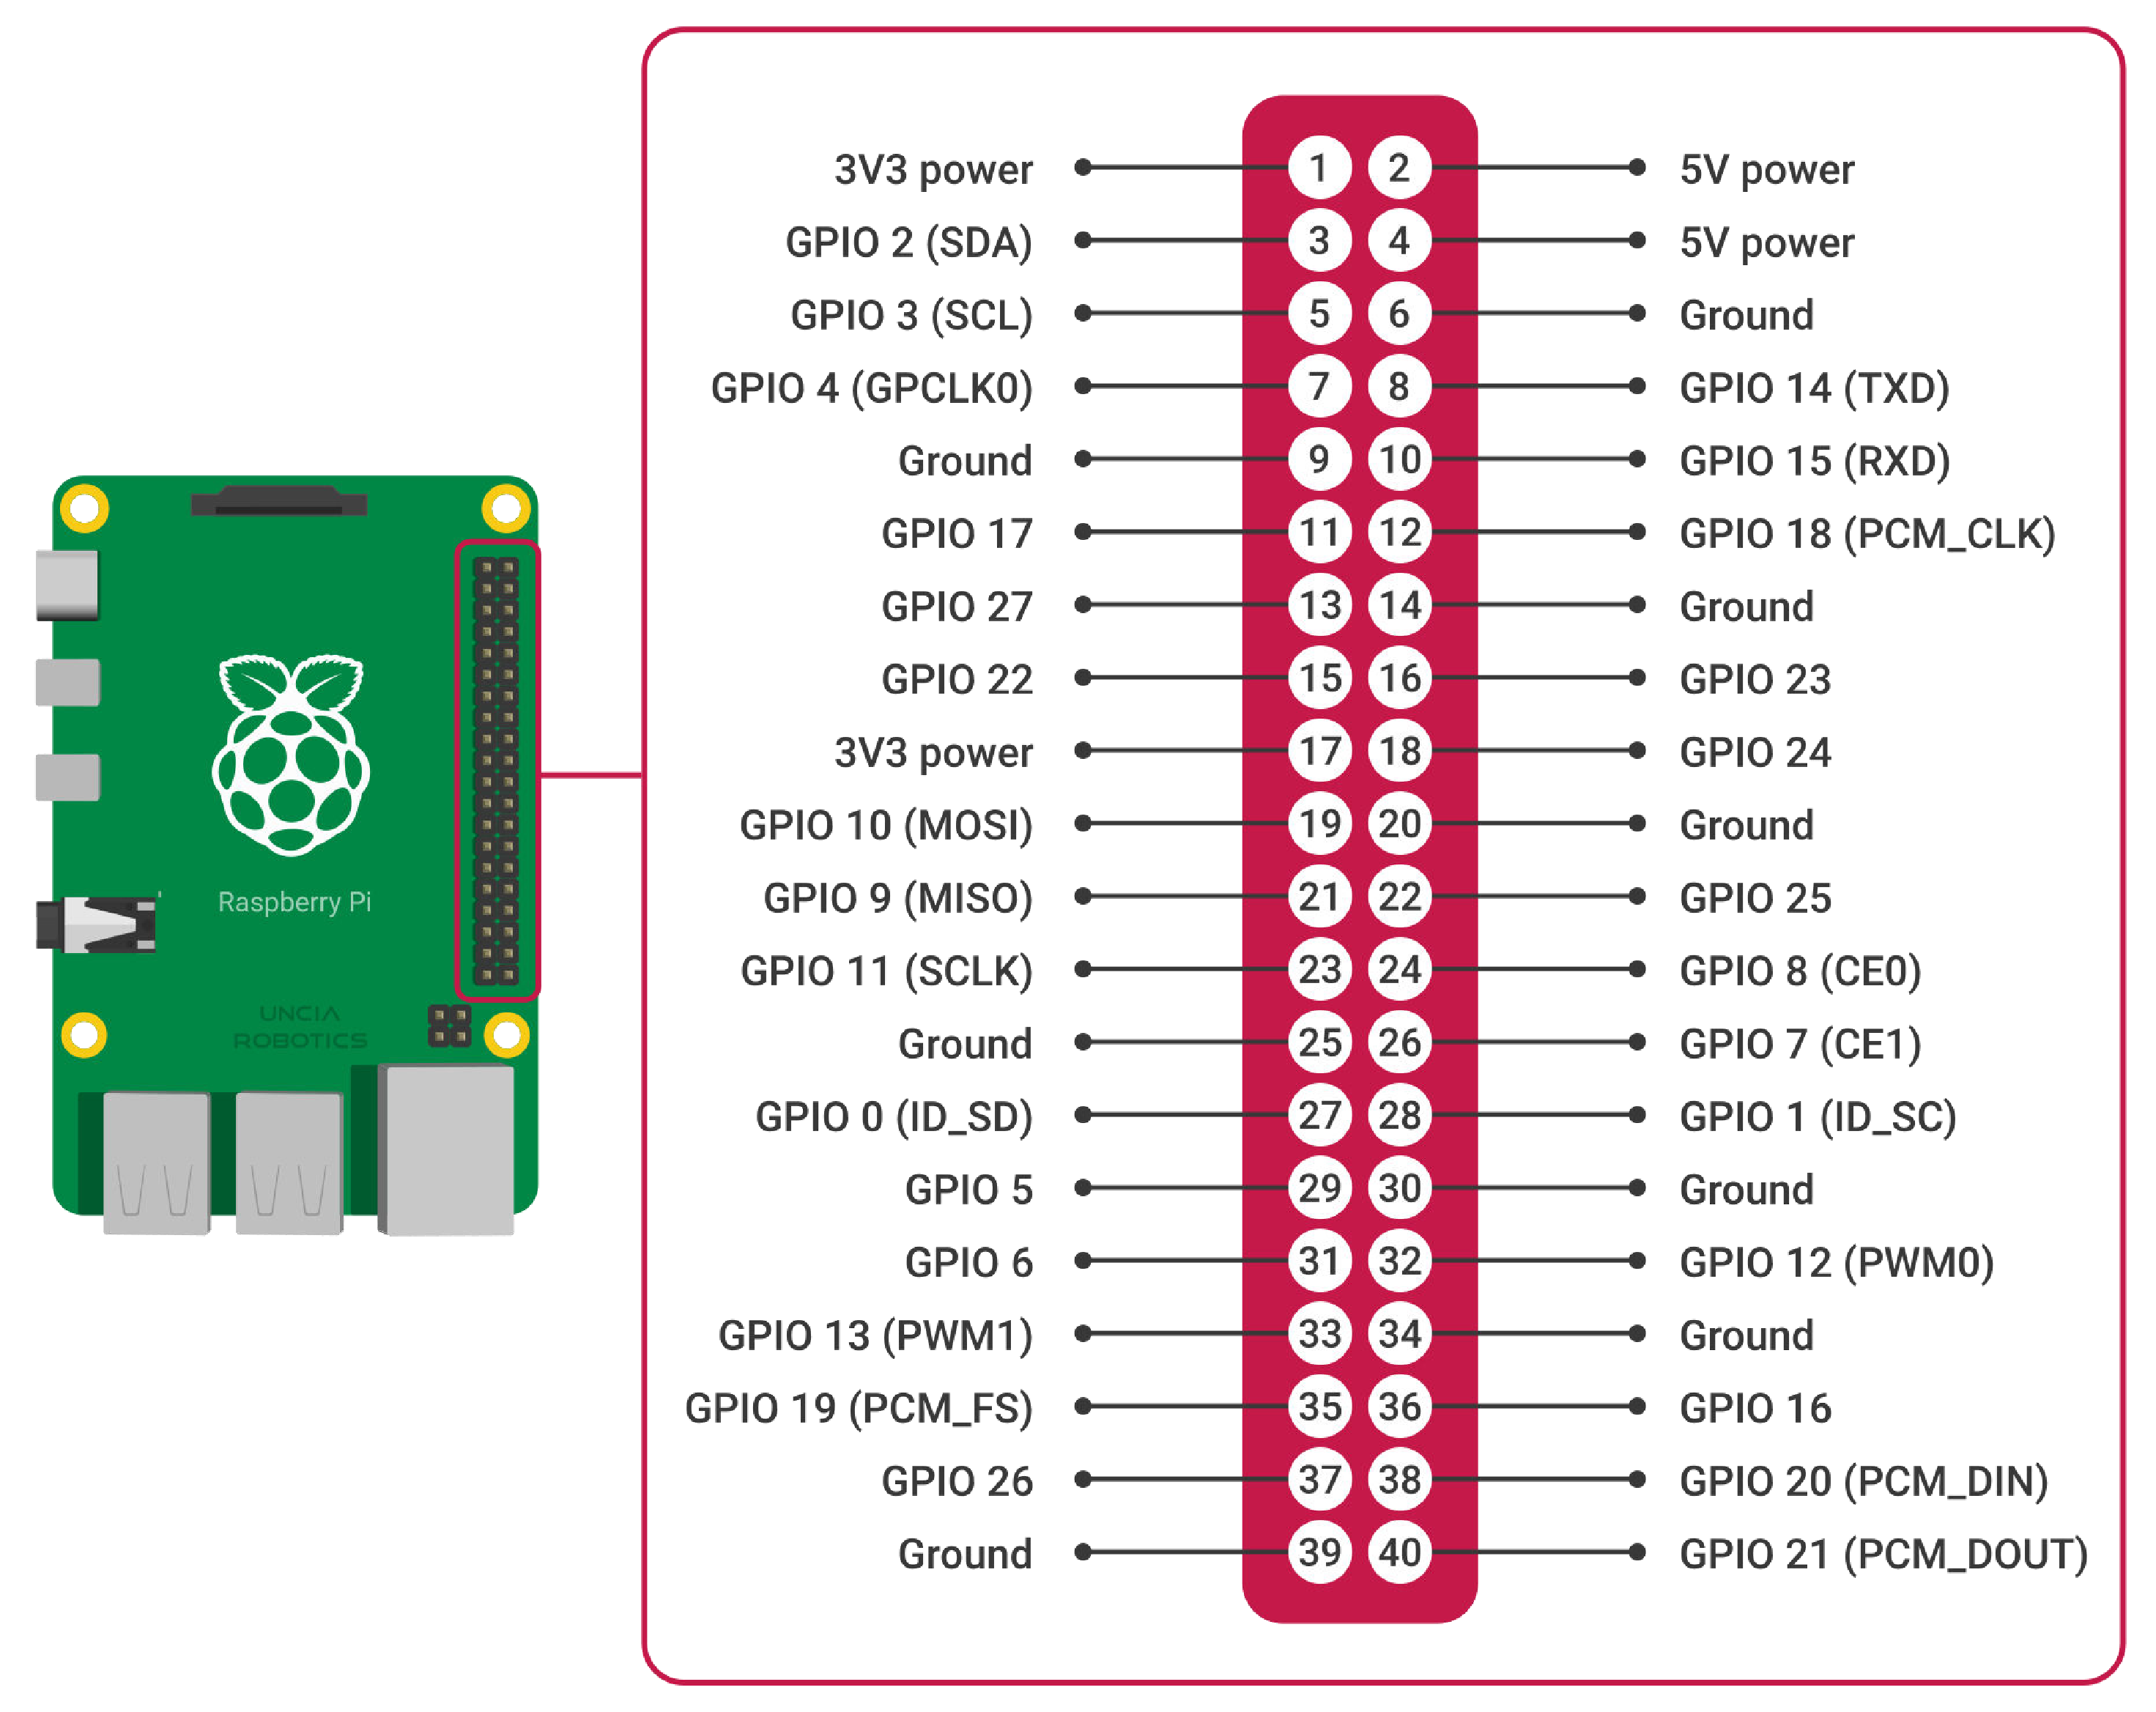
\includegraphics[width=15cm]{figures/Raspberry-Pinout.pdf}
	\vspace{-10pt}
	\caption{Arduino针脚}
	% \vspace{-10pt}
\end{figure}

\clearpage
\sectiontwo{B:Arduino Fritzing 图样\footnote[1]{图样与实际程序存在接线出入,可根据实际情况进行相应调整}}
\begin{figure}[!h]
	\centering
	% \vspace{-10pt}
	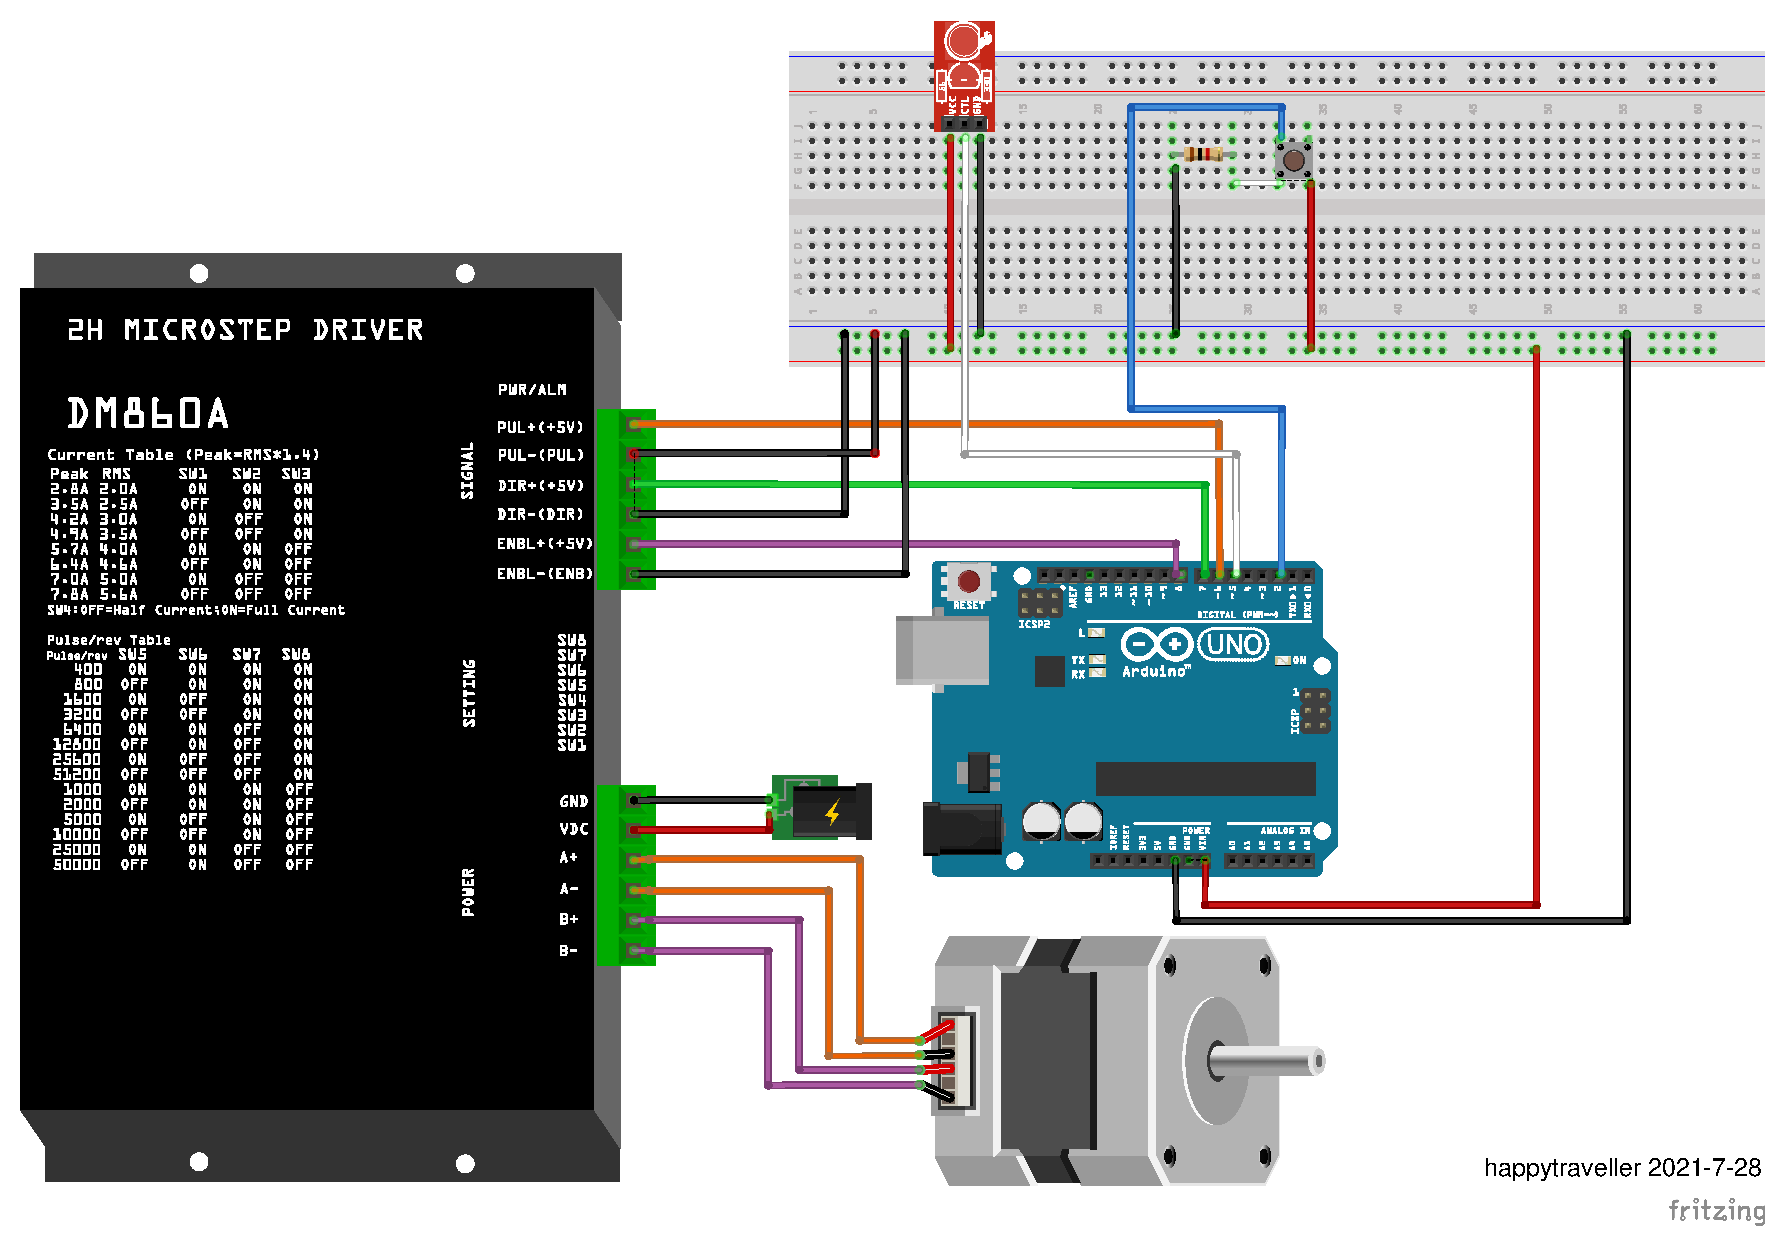
\includegraphics[width=14cm]{figures/直观图.pdf}
	\vspace{-10pt}
	\caption{实物接线图}
	% \vspace{-10pt}
\end{figure}

\begin{figure}[!h]
	\centering
	% \vspace{-10pt}
	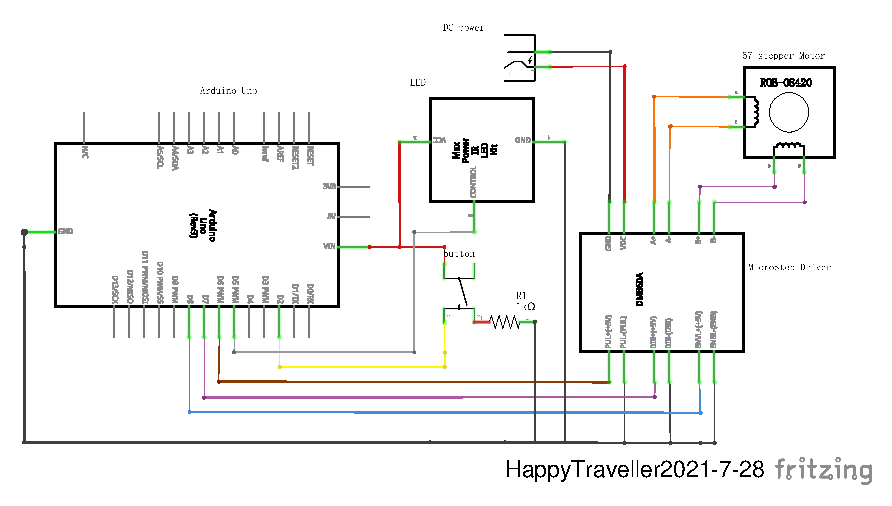
\includegraphics[width=14cm]{figures/Arduino 布线.pdf}
	\vspace{-10pt}
	\caption{针脚连接示意图}
	% \vspace{-10pt}
\end{figure}

运用Arduino对步进电机驱动的传动装置进行测试,元件包括:
传动装置、Microstep Driver(电机驱动板)、面包板、Arduino Uno R3
开发板、限位开关、数控LED灯、若干导线、直流电源。利用Arduino 官方IDE 进行
程序烧写。实现逻辑为传动块从靠近电机端移动到远离电机端,移动过程中不设置停留
限位开关中断触发后,传动块从远离电机端移动到靠近电机端,中途不停留,完成后,停等
一秒,而后重新执行远离电机程序。Arduino Uno仅设置2、3两个外部中断接口,参考附录A。
程序内容参考附录C。

直流电源供电12V、电流为0.6A,细分程度设置为2,衰减程度设置为20\%,电流设置
上限为1.5A,SW1-SW8的设置参数为(1,1,1,1,1,1,0,1)。参数的具体讲解参考附录C
\clearpage
% \columnseprule=3pt
\setlength{\columnsep}{1cm}
\begin{multicols*}{2}
	[
		\sectiontwo{C:程序参考及硬件参数介绍}
	]
	\lstinputlisting[
		style       =   C,
		caption     =   {\bf arduino.c},
		label       =   {arduino.c}
	]{Code/arduino.c}

	\vspace{0.5cm}

	\begin{wrapfigure}[12]{R}{0.22\textwidth}
		\centering
		\vspace{-10pt}
		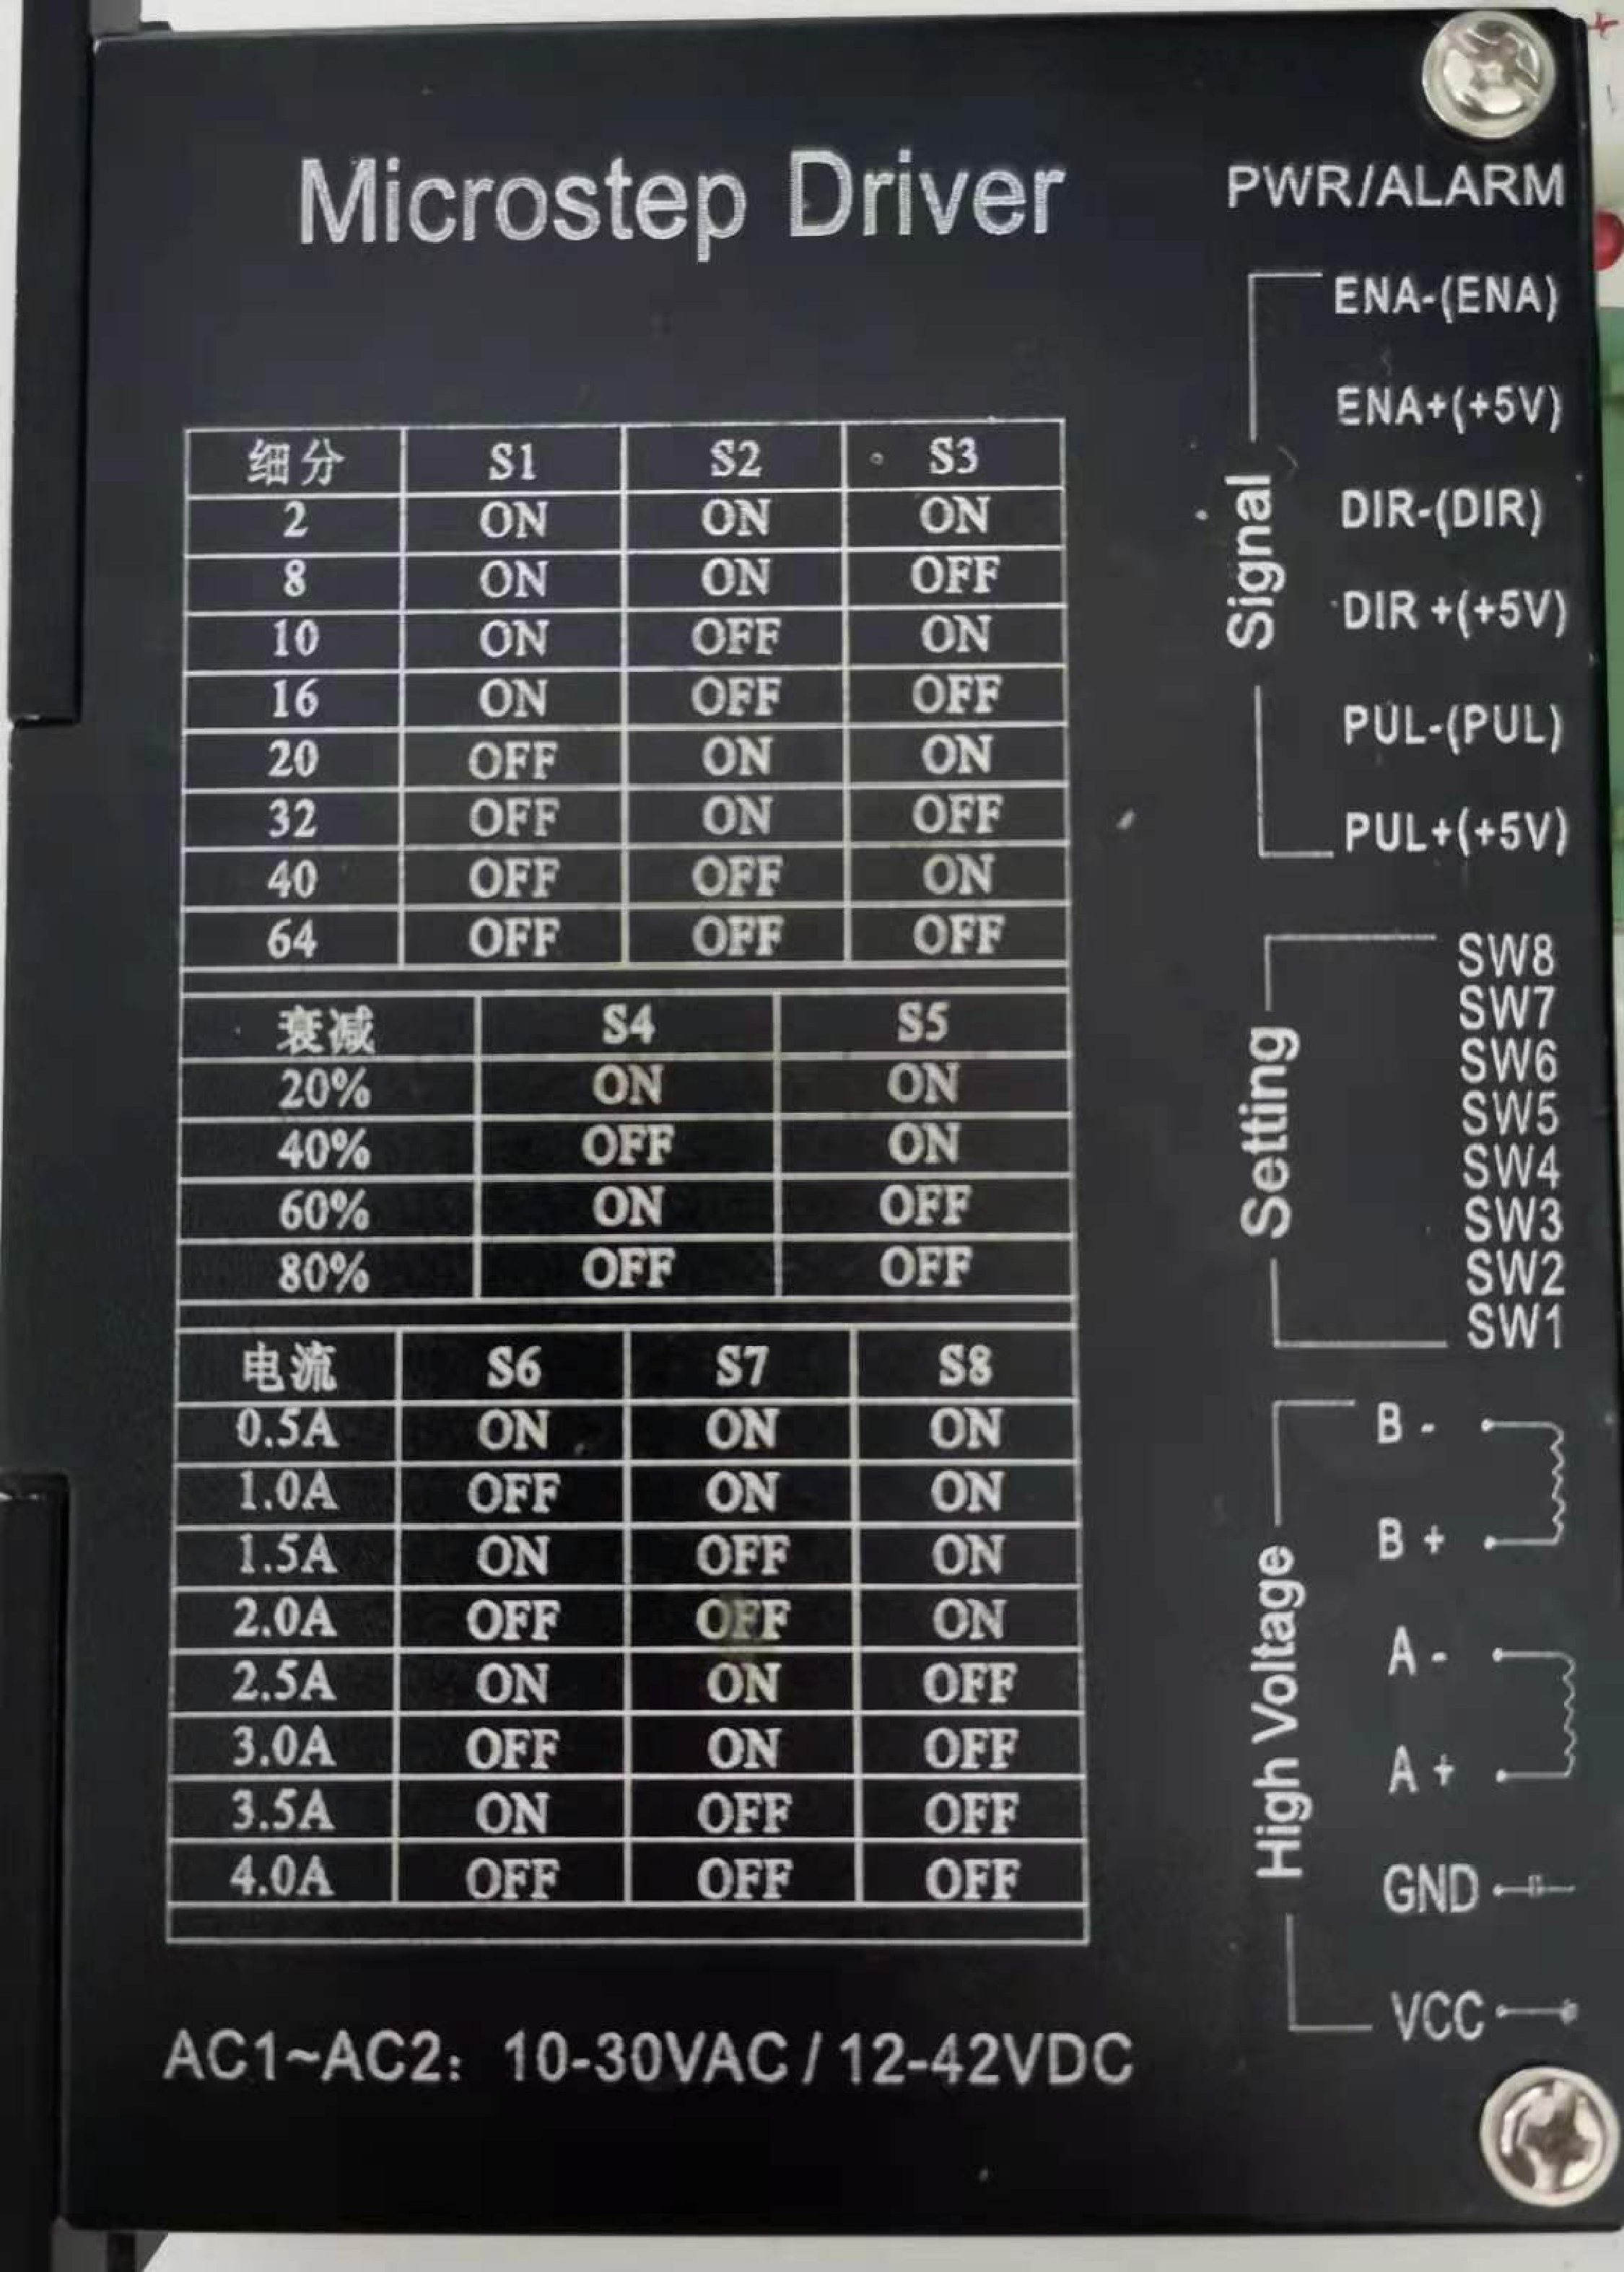
\includegraphics[width=3.7cm]{figures/硬件示意图.pdf}
		\vspace{-15pt}
		\caption{硬件参数说明}
		\vspace{-15pt}
	\end{wrapfigure}

	如右图所示,通过8个接口进行硬件参实的调节,其中SW1-SW3实现细分度的调整
	细分程度越高,单圈所需的脉冲次数也越多,在细分度为2的前提下,单圈脉冲次数
	为200。细分度共分为8级,分别为(2, 8, 10, 16, 20, 32, 40,64),在细分度为2的前提下,
	S1, S2, S3均置为ON(开启状态)。

	给电机线圈充电过程是线性的,当线圈的电流大于一定值的时候,单片机输入衰减时钟
	让电流达到稳定。快慢衰减是指在H桥中的选择场效应管的导通截至来控制电流放电速度
	的快慢,放电快则为快衰减,慢则为慢衰减。衰减程度共分为4级,分别为(20\%, 40\%, 60\%, 80\%)
	本次测试采用20\%慢速档。

	电流大小同样可分为8级,分别为(0.5A, 1.0A, 1.5A, 2.0A, 2.5A, 3.0A, 3.5A, 4.0A),本次测试
	采用1.5A档位。
\end{multicols*}
\clearpage
\sectiontwo{程序主界面}
\begin{figure}[!h]
	\centering
	% \vspace{-5pt}
	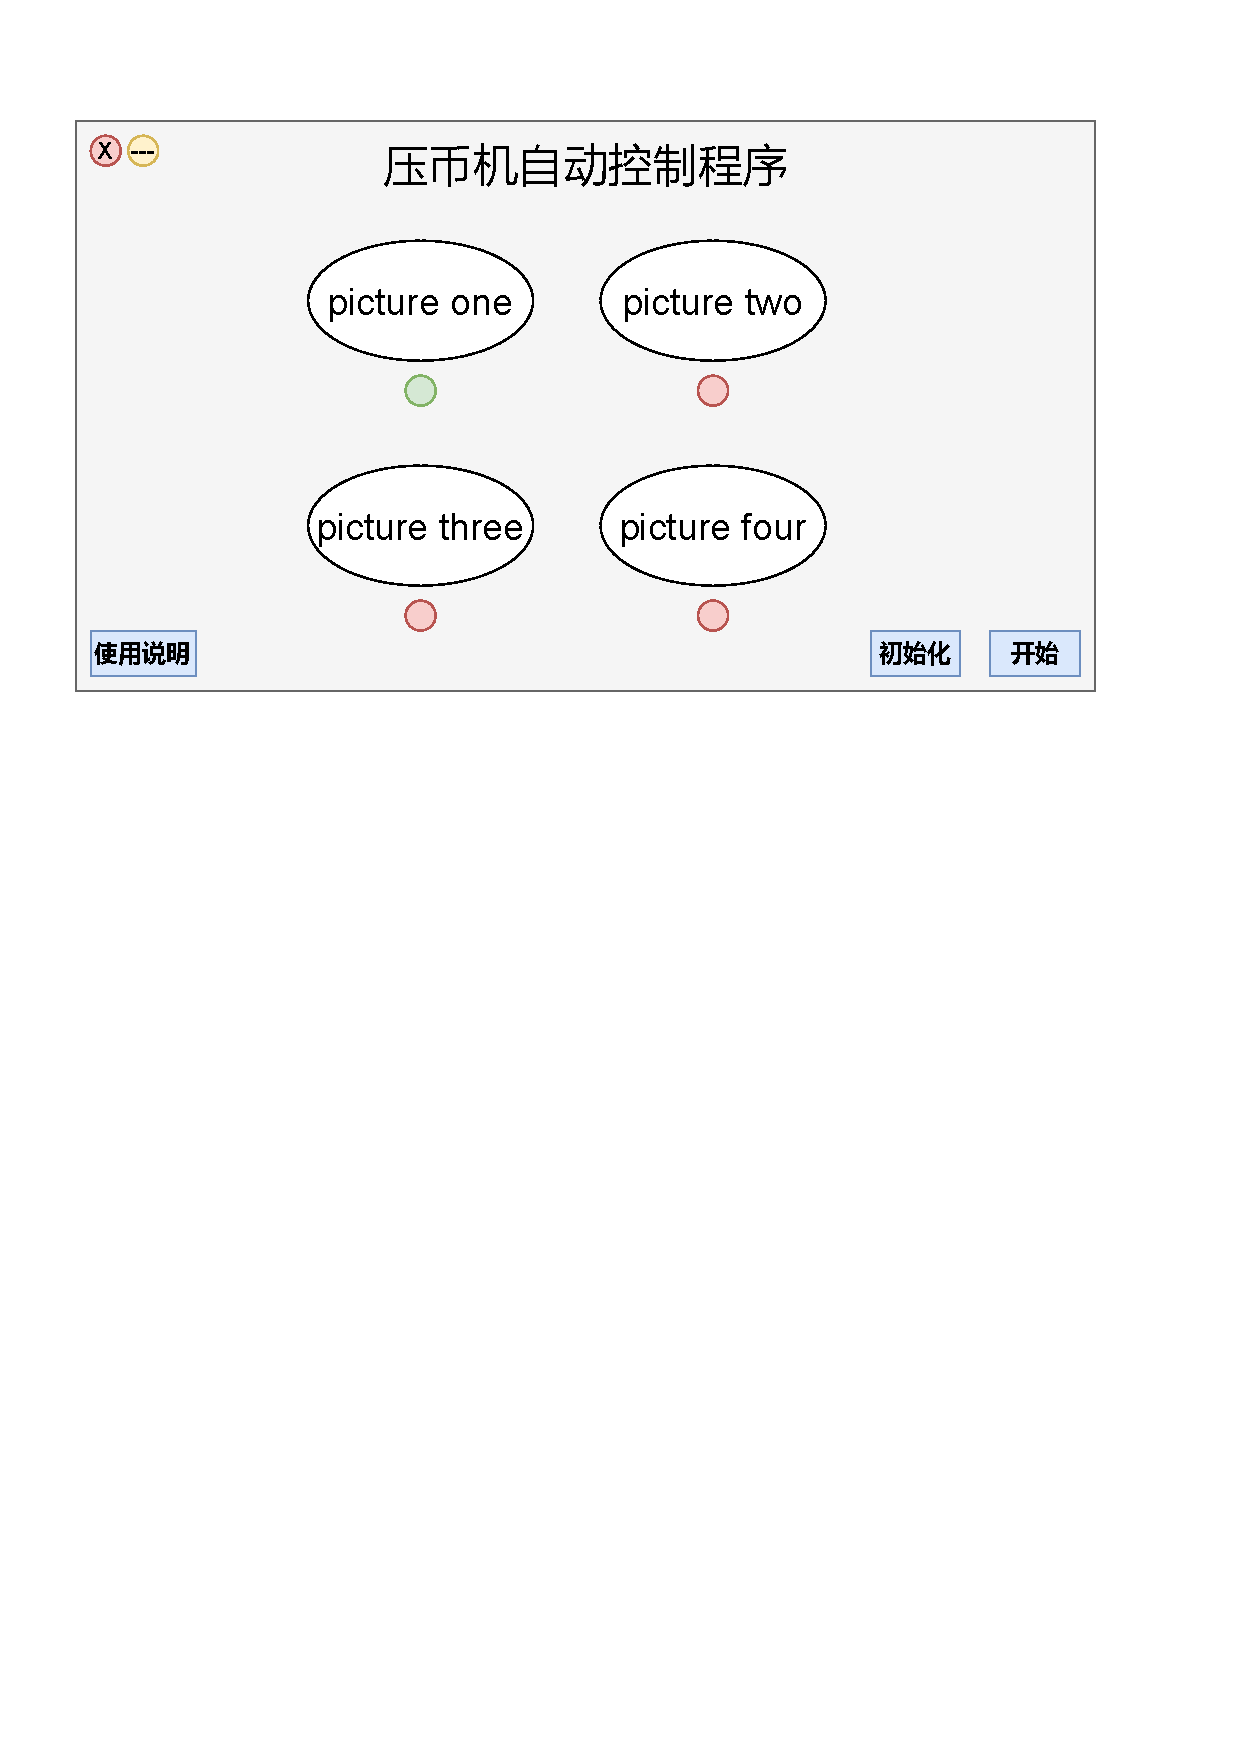
\includegraphics[width=16cm]{figures/界面开发.pdf}
	% \vspace{-10pt}
	\caption{程序主界面}
	% \vspace{-10pt}
\end{figure}


\clearpage
\sectionone{接口说明和功能说明}
\begin{multicols}{2}
	\sectiontwo{I2C}
	\begin{itemize}
		\item
	\end{itemize}
	\sectiontwo{SPI:串行外设接口}
	\begin{itemize}
		\item 概述\\
		      Raspberry Pi系列的设备配备了许多SPI总线。SPI可以用来
		      连接各种各样的外围设备--显示器、网络控制器(以太网、CAN
		      总线)、UART等等。
		\item 硬件支撑\\
		      所有Raspberry Pi设备共有的BCM2835内核有3个SPI控制器。

		      SPI0,在所有Pis的头部都有(尽管有一个替代的映射,只在计算模块上可用)。

		      SPI1,可用于40针版本的Pis。

		      SPI2,只适用于计算模块

		      BCM2711增加了另外4条SPI总线--SPI3至SPI6,每条都有2个硬件芯片选择。所有这些都可以在40针头上使用(只要没有其他东西试图使用相同的引脚)。
		\item 针脚替代说明图\\
		      \href{https://www.raspberrypi.org/documentation/hardware/raspberrypi/spi/README.md}{网站参考}
		\item 信号定义\\
		      - SCK : Serial Clock 串行时钟

		      - MOSI : Master Output,Slave Input 主发从收

		      - MISO : Master Input,Slave Output 主收从发

		      - SS/CS : Slave Select 片选信号
	\end{itemize}
\end{multicols}
\end{document}